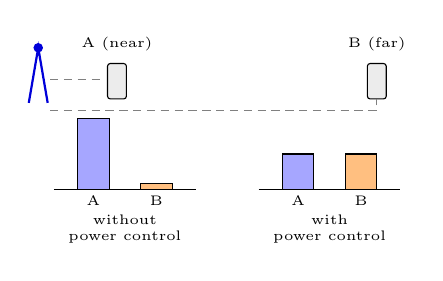
\begin{tikzpicture}[>=latex]
    \def\phone#1#2{\draw[fill=gray!15, rounded corners=1pt] ({#1-0.12},1.15) rectangle ({#1+0.12},1.6);
        \node[font=\tiny] at (#1,1.85) {#2};}

    % Base station and two terminals at different distances
    \draw[thick, blue!85!black] (-0.12,1.1) -- (0,1.8) -- (0.12,1.1);
    \filldraw[blue!85!black] (0,1.8) circle (1.5pt);
    \phone{1.0}{A (near)}
    \phone{4.3}{B (far)}
    \draw[densely dashed, gray] (0.15,1.4) -- (0.85,1.4);
    \draw[densely dashed, gray] (0.15,1.0) -- (4.3,1.0) -- (4.3,1.15);

    % Received uplink power at the base station
    \draw (0.2,0) -- (2.0,0);
    \draw[fill=blue!35] (0.5,0) rectangle (0.9,0.9);
    \draw[fill=orange!50] (1.3,0) rectangle (1.7,0.08);
    \node[font=\tiny] at (0.7,-0.15) {A};
    \node[font=\tiny] at (1.5,-0.15) {B};
    \node[font=\tiny, align=center] at (1.1,-0.5) {without\\power control};

    \draw (2.8,0) -- (4.6,0);
    \draw[fill=blue!35] (3.1,0) rectangle (3.5,0.45);
    \draw[fill=orange!50] (3.9,0) rectangle (4.3,0.45);
    \node[font=\tiny] at (3.3,-0.15) {A};
    \node[font=\tiny] at (4.1,-0.15) {B};
    \node[font=\tiny, align=center] at (3.7,-0.5) {with\\power control};
\end{tikzpicture}
